\section{Generator map}
\label{ch:mazegen}

W rozdziale \ref{ch:tests} opisano wyniki testów przeprowadzonych na losowo wygenerowanych środowiskach.
Do ich automatycznego utworzenia wykorzystano własny generator map, który zapewnia im pewne pożądane własności opisane poniżej.

Zastosowanie zwykłego losowania położenia przeszkód na mapie mogłoby spowodować, że do niektórych obszarów na mapie nie udałoby się znaleźć drogi, nawet mimo braku istnienia pozostałych agentów. Takie środowisko nie miałoby sensownego zastosowania w praktyce, w kooperacyjnym znajdowaniu tras.

Zależy nam, aby uzyskać środowisko cechujące się dużą liczbą przeszkód i wąskimi korytarzami, aby uwypuklić problem występowania wąskich gardeł. Jednocześnie chcemy jednak, aby istniała możliwość przejścia między dwoma dowolnymi punktami na mapie.
Do rozwiązania problemu wygenerowania takich labiryntów posłużymy się teorią grafów i pojęciem grafu spójnego.

\begin{definition}{\bf Graf spójny\\}
	Graf spójny spełnia warunek, że dla każdej pary wierzchołków istnieje łącząca je ścieżka.
\end{definition}

Układ pól na mapie będziemy reprezentować jako graf.
W naszym przypadku wszystkie przejezdne pola na mapie są wierzchołkami grafu. Natomiast połączenia między sąsiednimi przejezdnymi polami (między którymi istnieje możliwość bezpośredniego przejścia) są krawędziami w grafie.

Aby zapewnić, że powstały graf będzie spójny, na początku losujemy jedno pole będące ziarnem rozrostu labiryntu, a następnie do takiego podgrafu dołączamy kolejne wierzchołki, łącząc je drogą na mapie. Krok ten powtarzamy do momentu, aż wszystkie wierzchołki zostaną dołączone.
W tym celu wykorzystamy dwie pomocnicze listy wierzchołków:
\begin{itemize}
	\item lista wierzchołków {\it odwiedzonych} - zawiera wierzchołki (pola) należące już do labiryntu. Między wszystkimi wierzchołkami z listy {\it odwiedzonych} istnieje łącząca je droga, tworzą one graf spójny.
	\item lista wierzchołków {\it nieodwiedzonych} - zawiera nieodwiedzone wierzchołki (pola), które nie zostały jeszcze dołączone do labiryntu.
\end{itemize}

Kolejne kroki algorytmu przedstawiają się następująco:
\begin{enumerate}
	\item Inicjalizacja pustych list wierzchołków: {\it odwiedzonych} i {\it nieodwiedzonych}.
	\item Zapełnienie całej mapy przeszkodami.
	\item Zaznaczenie co drugiego pola (wzdłuż każdego z wymiarów) jako wolne (por. rys. \ref{fig:etapy-generowania}a) i dodanie ich do listy {\it nieodwiedzonych}.
	\item Wylosowanie ziarna rozrostu labiryntu z listy {\it nieodwiedzonych}, przeniesienie go na listę {\it odwiedzonych}.
	\item Łączenie kolejnych wierzchołków nieodwiedzonych z wierzchołkami odwiedzonymi. Dopóki lista {\it nieodwiedzonych} nie jest pusta:
	\begin{enumerate}
		\item Wylosowanie wierzchołka z listy {\it nieodwiedzonych}.
		\item Znalezienie najbliższego dla niego (w sensie metryki miejskiej) sąsiada z listy {\it odwiedzonych}.
		\item Połączenie wierzchołków drogą poprzez "wyburzanie" przeszkód (zaznaczania pola jako wolne) przy przesuwaniu się w kierunku wierzchołka docelowego, najpierw wzdłuż osi poziomej, następnie wzdłuż osi pionowej (por. rys. \ref{fig:etapy-generowania}b).
	\end{enumerate}
\end{enumerate}

Pojedyncze dołączanie kolejnych wierzchołków do rozrastającego się grafu labiryntu zapewnia, że wynikowy graf również będzie grafem spójnym.

Poniżej przedstawiono pseudokod, obrazujący szczegóły działania zaproponowanej metody.

\begin{algorithm}[H]
	\caption{Generowanie labiryntu}\label{alg:mazegen}
  \begin{algorithmic}[1]
\Require {$w$ - szerokość mapy, $h$ - wysokość mapy}

\State $mapa[][] \gets$ nowa tablica $w \times h$ wypełniona wartościami $ZABLOKOWANE$

\State $nieodwiedzone \gets \varnothing$ \Comment{Inicjalizacja pustych list}
\State $odwiedzone \gets \varnothing$
\For{$x \gets 0$; $x < w$; $x \gets x + 2$} \Comment{co drugi indeks szerokości}
	\For{$y \gets 0$; $y < h$; $y \gets y + 2$} \Comment{co drugi indeks wysokości}
		\State $mapa[x][y] \gets WOLNE$
		\State dodaj $mapa[x][y]$ do $nieodwiedzone$
	\EndFor
\EndFor

\State $ziarno$ $\gets$ losowe pole z $nieodwiedzone$
\State dodaj $ziarno$ do $odwiedzone$
\State usuń $ziarno$ z $nieodwiedzone$

\While{$nieodwiedzone \ne \varnothing$} \Comment{dopóki $nieodwiedzone$ nie jest pusta}
	\State $nowePole$ $\gets$ losowe pole z $nieodwiedzone$
	\State $sasiad$ $\gets$ \Call{znajdźNajbliższegoSąsiada}{$odwiedzone$, $nowePole$}
	\State \Call{wyburzDrogę}{$mapa$, $nowePole$, $sasiad$}
	\State dodaj $nowePole$ do $odwiedzone$
	\State usuń $nowePole$ z $nieodwiedzone$
\EndWhile

\State {\bf return} $mapa[][]$

\State 
\Function{wyburzDrogę}{$mapa$, $poleZ$, $poleDo$}
	\State $x \gets poleZ.x$
	\State $y \gets poleZ.y$
	\While{$x < poleDo.x$} \Comment{Przesuwanie w prawo}
		\State $mapa[x\verb-++-][y] \gets WOLNE$ 
	\EndWhile
	\While{$x > poleDo.x$} \Comment{Przesuwanie w lewo}
		\State $mapa[x\verb+--+][y] \gets WOLNE$
	\EndWhile
	\While{$y < poleDo.y$} \Comment{Przesuwanie w dół}
		\State $mapa[x][y\verb-++-] \gets WOLNE$
	\EndWhile
	\While{$y > poleDo.y$} \Comment{Przesuwanie w górę}
		\State $mapa[x][y\verb+--+] \gets WOLNE$
	\EndWhile
\EndFunction
  \end{algorithmic}
\end{algorithm}

Oznaczenie $x\verb-++-$ oraz $x\verb+--+$ oznacza odpowiednio postinkrementację i postdekrementację (dokonanie zwiększenia lub zmniejszenia o 1 {\bf po} wykorzystaniu wartości zmiennej w wyrażeniu).
Funkcja {\it znajdźNajbliższegoSąsiada} wyszukuje sąsiada dla pola $nowePole$ z listy $odwiedzone$. Wynik wyszukiwania jest najbliższy w sensie metryki miejskiej (metryki Manhattan).

Kolejne etapy generowania labiryntu zobrazowano na rysunku \ref{fig:etapy-generowania}.

\begin{figure}
    \centering
        \subfloat[]{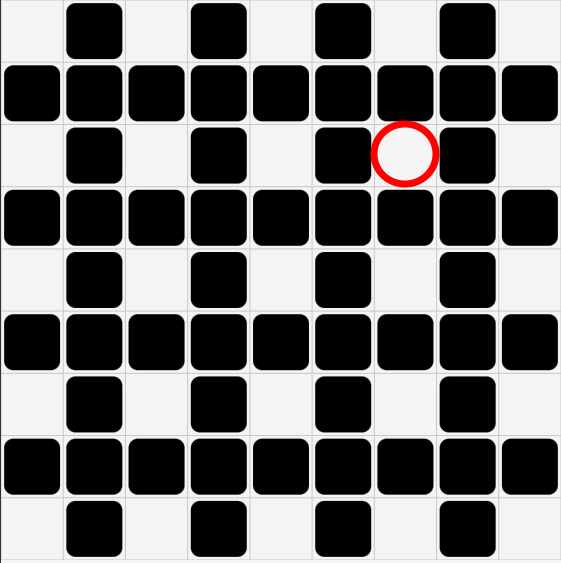
\includegraphics[width=0.3\columnwidth]{img/mazegen/maze-0initial-marks}}
        \qquad
        \subfloat[]{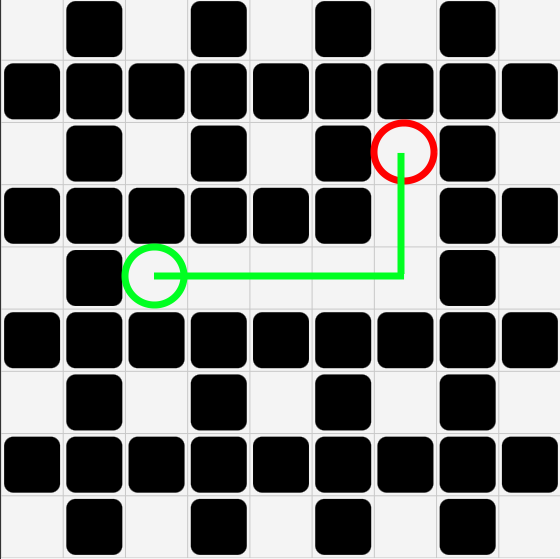
\includegraphics[width=0.3\columnwidth]{img/mazegen/maze-1cycle-marks}}
        \qquad
        \subfloat[]{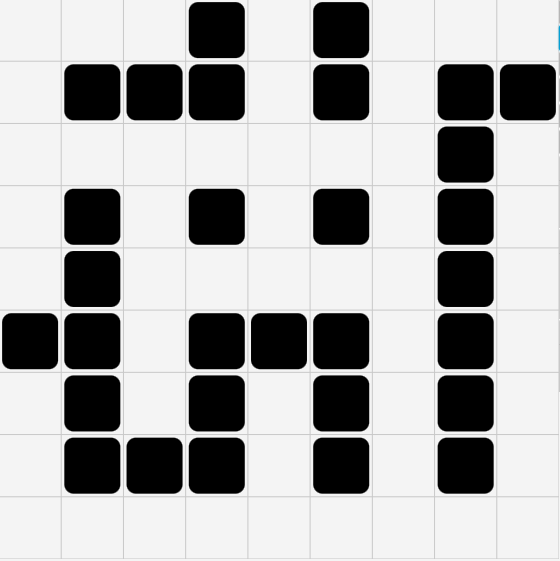
\includegraphics[width=0.3\columnwidth]{img/mazegen/maze-result}}
    \caption{Kolejne etapy generowania labiryntu.
    (a) Zaznaczenie co drugiego pola jako wolne i wybór ziarna rozrostu labiryntu.
    (b) Wylosowanie i łączenie kolejnego wierzchołka poprzez "wyburzanie" przeszkód na drodze
    (c) Wynikowa mapa pochodząca z generatora}
    \label{fig:etapy-generowania}
\end{figure}

Na rysunku \ref{fig:maze75-75} przedstawiono przykładowy labirynt wygenerowany opisanym algorytmem.
\begin{figure}
	\centering
	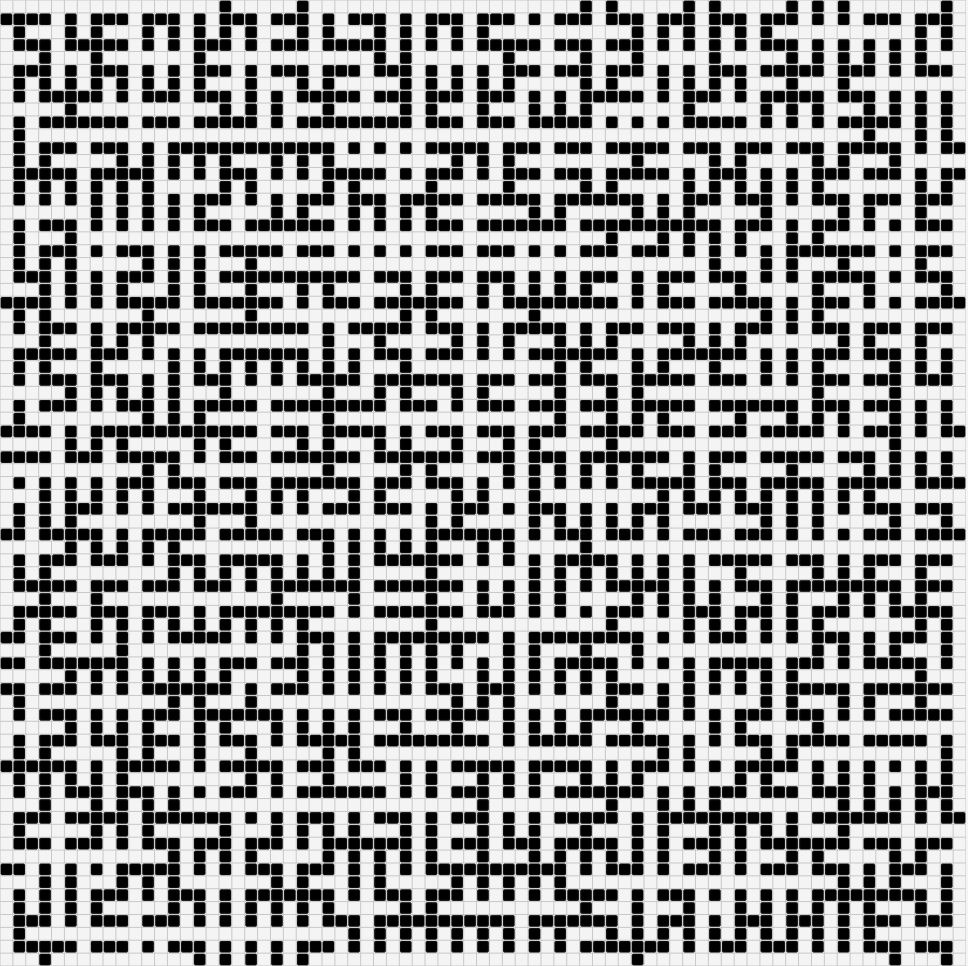
\includegraphics[width=0.6\columnwidth]{img/mazegen/maze-75-75}
	\caption{Przykładowy labirynt rozmiaru $75 \times 75$ pochodzący z generatora map}
	\label{fig:maze75-75}
\end{figure}

Wygenerowane w ten sposób mapy mają jeszcze jedną właściwość - w takim środowisku robot nie ma nigdy możliwości wykonania ruchu ukośnego (innego niż w poziomie lub pionie). Pozwala to wprowadzić pewne ograniczenia do niektórych algorytmów planowania (por. \ref{ch:theory-coop-astar}), które przyspieszają wykonywanie obliczeń ze względu na możliwość założenia jednakowego czasu trwania wszystkich ruchów robotów. Nie będziemy jednak tego zakładać na tym etapie, gdyż chcemy, aby opracowana metoda planowania tras mogła także działać w środowiskach innego typu.
